\section{Mobile development}

This section outlines the tools and methods the group discussed for how to
develop the game for both Android and iOS.

\subsection{Native}

Developing the application natively for both Android and iOS would allow us more
direct control over the behavior, appearance and performance of the application.
However, then we would have to develop in both Java and Objective-C in parallel,
with all the trouble that would cause not even considering other platform
differences. It is unlikely that we will be able to finish developing if we were
to develop natively.

\subsection{Cross Platform Frameworks}

Here we outline the cross platform frameworks we considered to let us develop for
both Android and iOS without having to maintain two code bases.

\paragraph{PhoneGap}
PhoneGap takes applications written with web technologies and wraps them in
a different ``web view'' application for each of the mobile platforms you
target. In essence, it's like saving a web page on your phone and opening
it in a browser without window chrome. This allows you to ``write once, run
everywhere''. Additionally, the PhoneGap framework wraps the native APIs of
different platforms in a single JavaScript API which is made available to
developers using PhoneGap. This makes PhoneGap apps potentially much more
powerful than simple web pages. \cite{phonegapAbout}

\paragraph{Corona}

Corona is a software development kit (SDK) which allows developers to build
applications for iPhone, iPad, Android and other devices. Corona is not open
source and costs money to use. Corona also enforces a monthly revenue limit for
developers unless they use the most expensive pricing plans\cite{coronaPrice}.
Corona lets programmers develop using Lua.\cite{coronaSDK} Advantages to using
Corona is that it comes with quite a bit of handy tools for developing video
games, but Corona is also quite costly and not open source.

\subsection{JavaScript Libraries}

Because Phonegap seemed like the stronger candidate for cross platform development, 
we also had to consider which JavaScript libraries we were going to use, because
Phonegap doesn't come with any tools for JavaScript development, just the means 
to do cross platform.

\paragraph{Backbone.js}
The JavaScript programming language does not strictly enforce any specific
architecture or code organization. Furthermore, JavaScript was initially
created so that simple interaction could be added to web pages when the web was
still an immature platform. These two factors led to a long history of poorly
structured JavaScript, or ``spaghetti code''.

Backbone.js attempts to solve this problem by introducing the MVP
(model--view--presenter) software pattern to client-side applications,
separating domain data and logic (Backbone models) from the user interface
(HTML) and mediating between the two through a presenter (Backbone view).

Backbone.js is widely used in industry and has only one dependency, the
Underscore.js library which shares the same creator as Backbone.js.
Therefore it meets our customer's requirement that we use well known
technologies that can be easily maintained. \cite{backbone}

\paragraph{Jasmine}
Jasmine is a unit testing framework for JavaScript. It advocates BDD
(behavior-driven development) in that its syntax is descriptive of what the
tested code is supposed to do and reads like a user story. Like Backbone.js,
Jasmine is widely used in industry. It is also included by default when you
create a new PhoneGap project, so presumably the two fit nicely together.
\cite{jasmine}

\subsection{Conclusions}
Prior to this project, none of the team members had much previous experience
with writing mobile applications, and certainly not cross-platform ones.
Therefore, we looked for a framework to help us do this in a way that wouldn't
require us to write and maintain two completely seperate codebases for Android
and iOS. PhoneGap is one very popular such framework, and so from researching
different tools on the Internet, it seemed a sensible choice.

Having decided on using PhoneGap, the logical next step was to decide on some
frameworks to help us organize our JavaScript code. Once again, Backbone.js is
a very popular framework, and also one that a team member had some previous
knowledge of. It is a fairly light-weight framework in that it does not contain
a lot of ``magic''; it is more of an organizational aid than an expansive
toolset of its own, and so it was not too time-consuming to learn.

None of the team members had written automated tests in JavaScript previously,
so the choice of Jasmine as a testing framework was based mostly on searching
the Internet and asking friends with more experience in the area. It also
helped that a Jasmine template is included by default in new PhoneGap projects.

\begin{figure}[!ht]
\centering

\subfigure{
  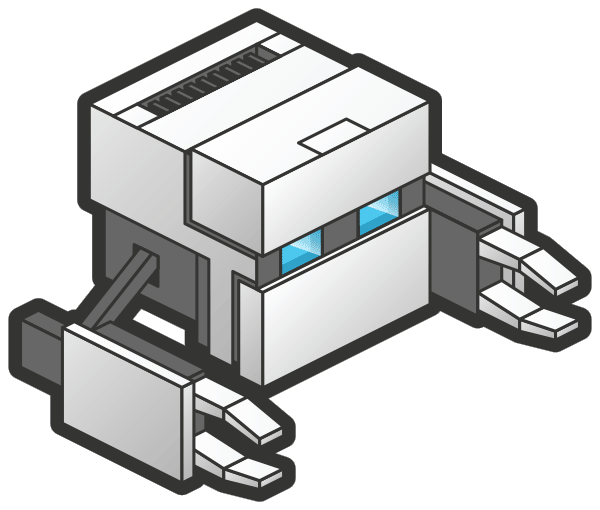
\includegraphics[scale=0.15]{pictures/phonegap}
}
\subfigure{
  
\includegraphics[scale=0.15]{pictures/backbone}
}
\subfigure{
  
\includegraphics[scale=0.9]{pictures/jasmine}
}
\caption{Phonegap, Backbone and Jasmine}
\end{figure}
